%!TEX root = thesis.tex

\section{Motivation}
\subsection{Energy Crisis, Resources and Climate Change}
The energy crisis is one of the most essential and critical crises in the 21st century. Due to the growth of population and the increase of energy intensity per capita, a shortage of energy supply has occurred frequently in recent years, which often causes an energy crisis, usually involving scarcity of oil, electricity or other natural resources. Nowadays, non-renewable resource still consists of a large proportion in the energy system. According to BP Statistical Review of World Energy \& Ember (see Figure~\ref{intro_renewable}), the share of electricity production from renewables has continued growing since 2007. In 2020, the share of electricity production from renewables was around 29\% (see Figure~\ref{intro_renewable}). In other words, non-renewasbles are still the majority sources of electricity production today, although the share of them is shrinking.\\


\begin{figure}
\center
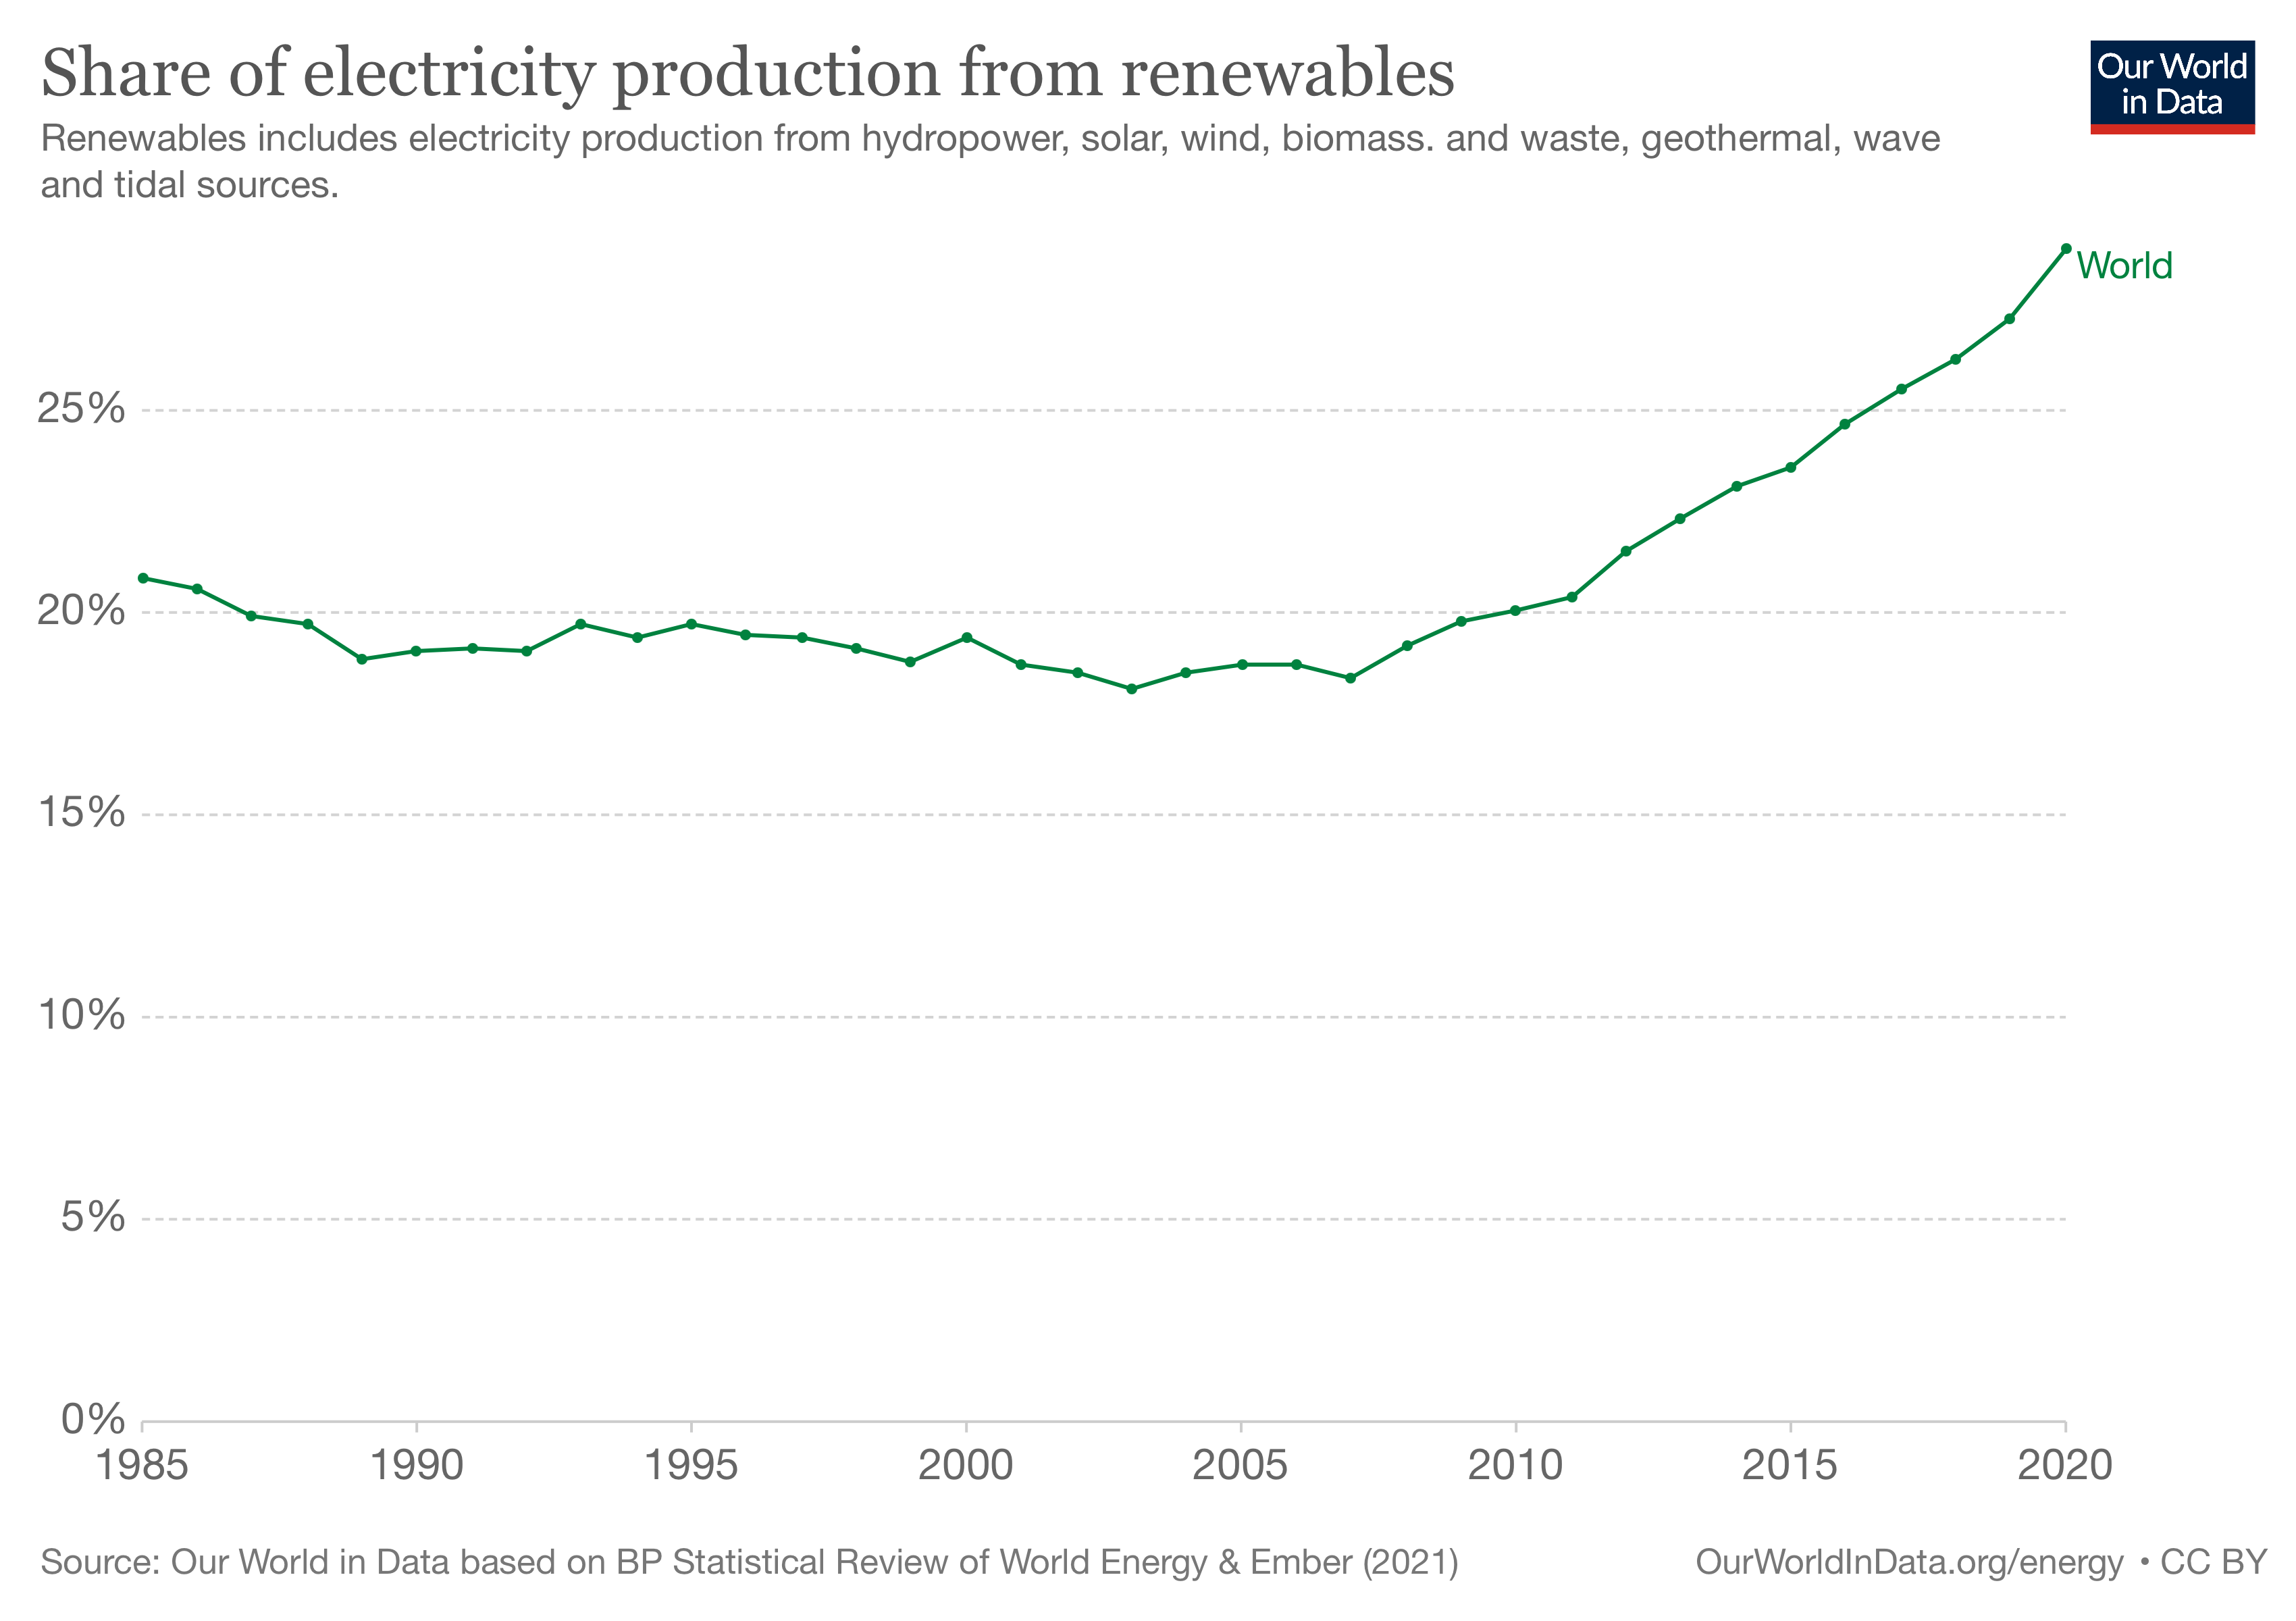
\includegraphics[scale=0.11]{img/intro_renewable.png}
\caption{The share of electricity production from renewables increased from around 18\% to 21\% during 1985 to 2007~\cite{BP2021bp}. The share of electricity production from renewables has been continued growing since 2007. In 2020, the share of electricity production from renewables was around 29\%.}
\label{intro_renewable} % Figure 1.1

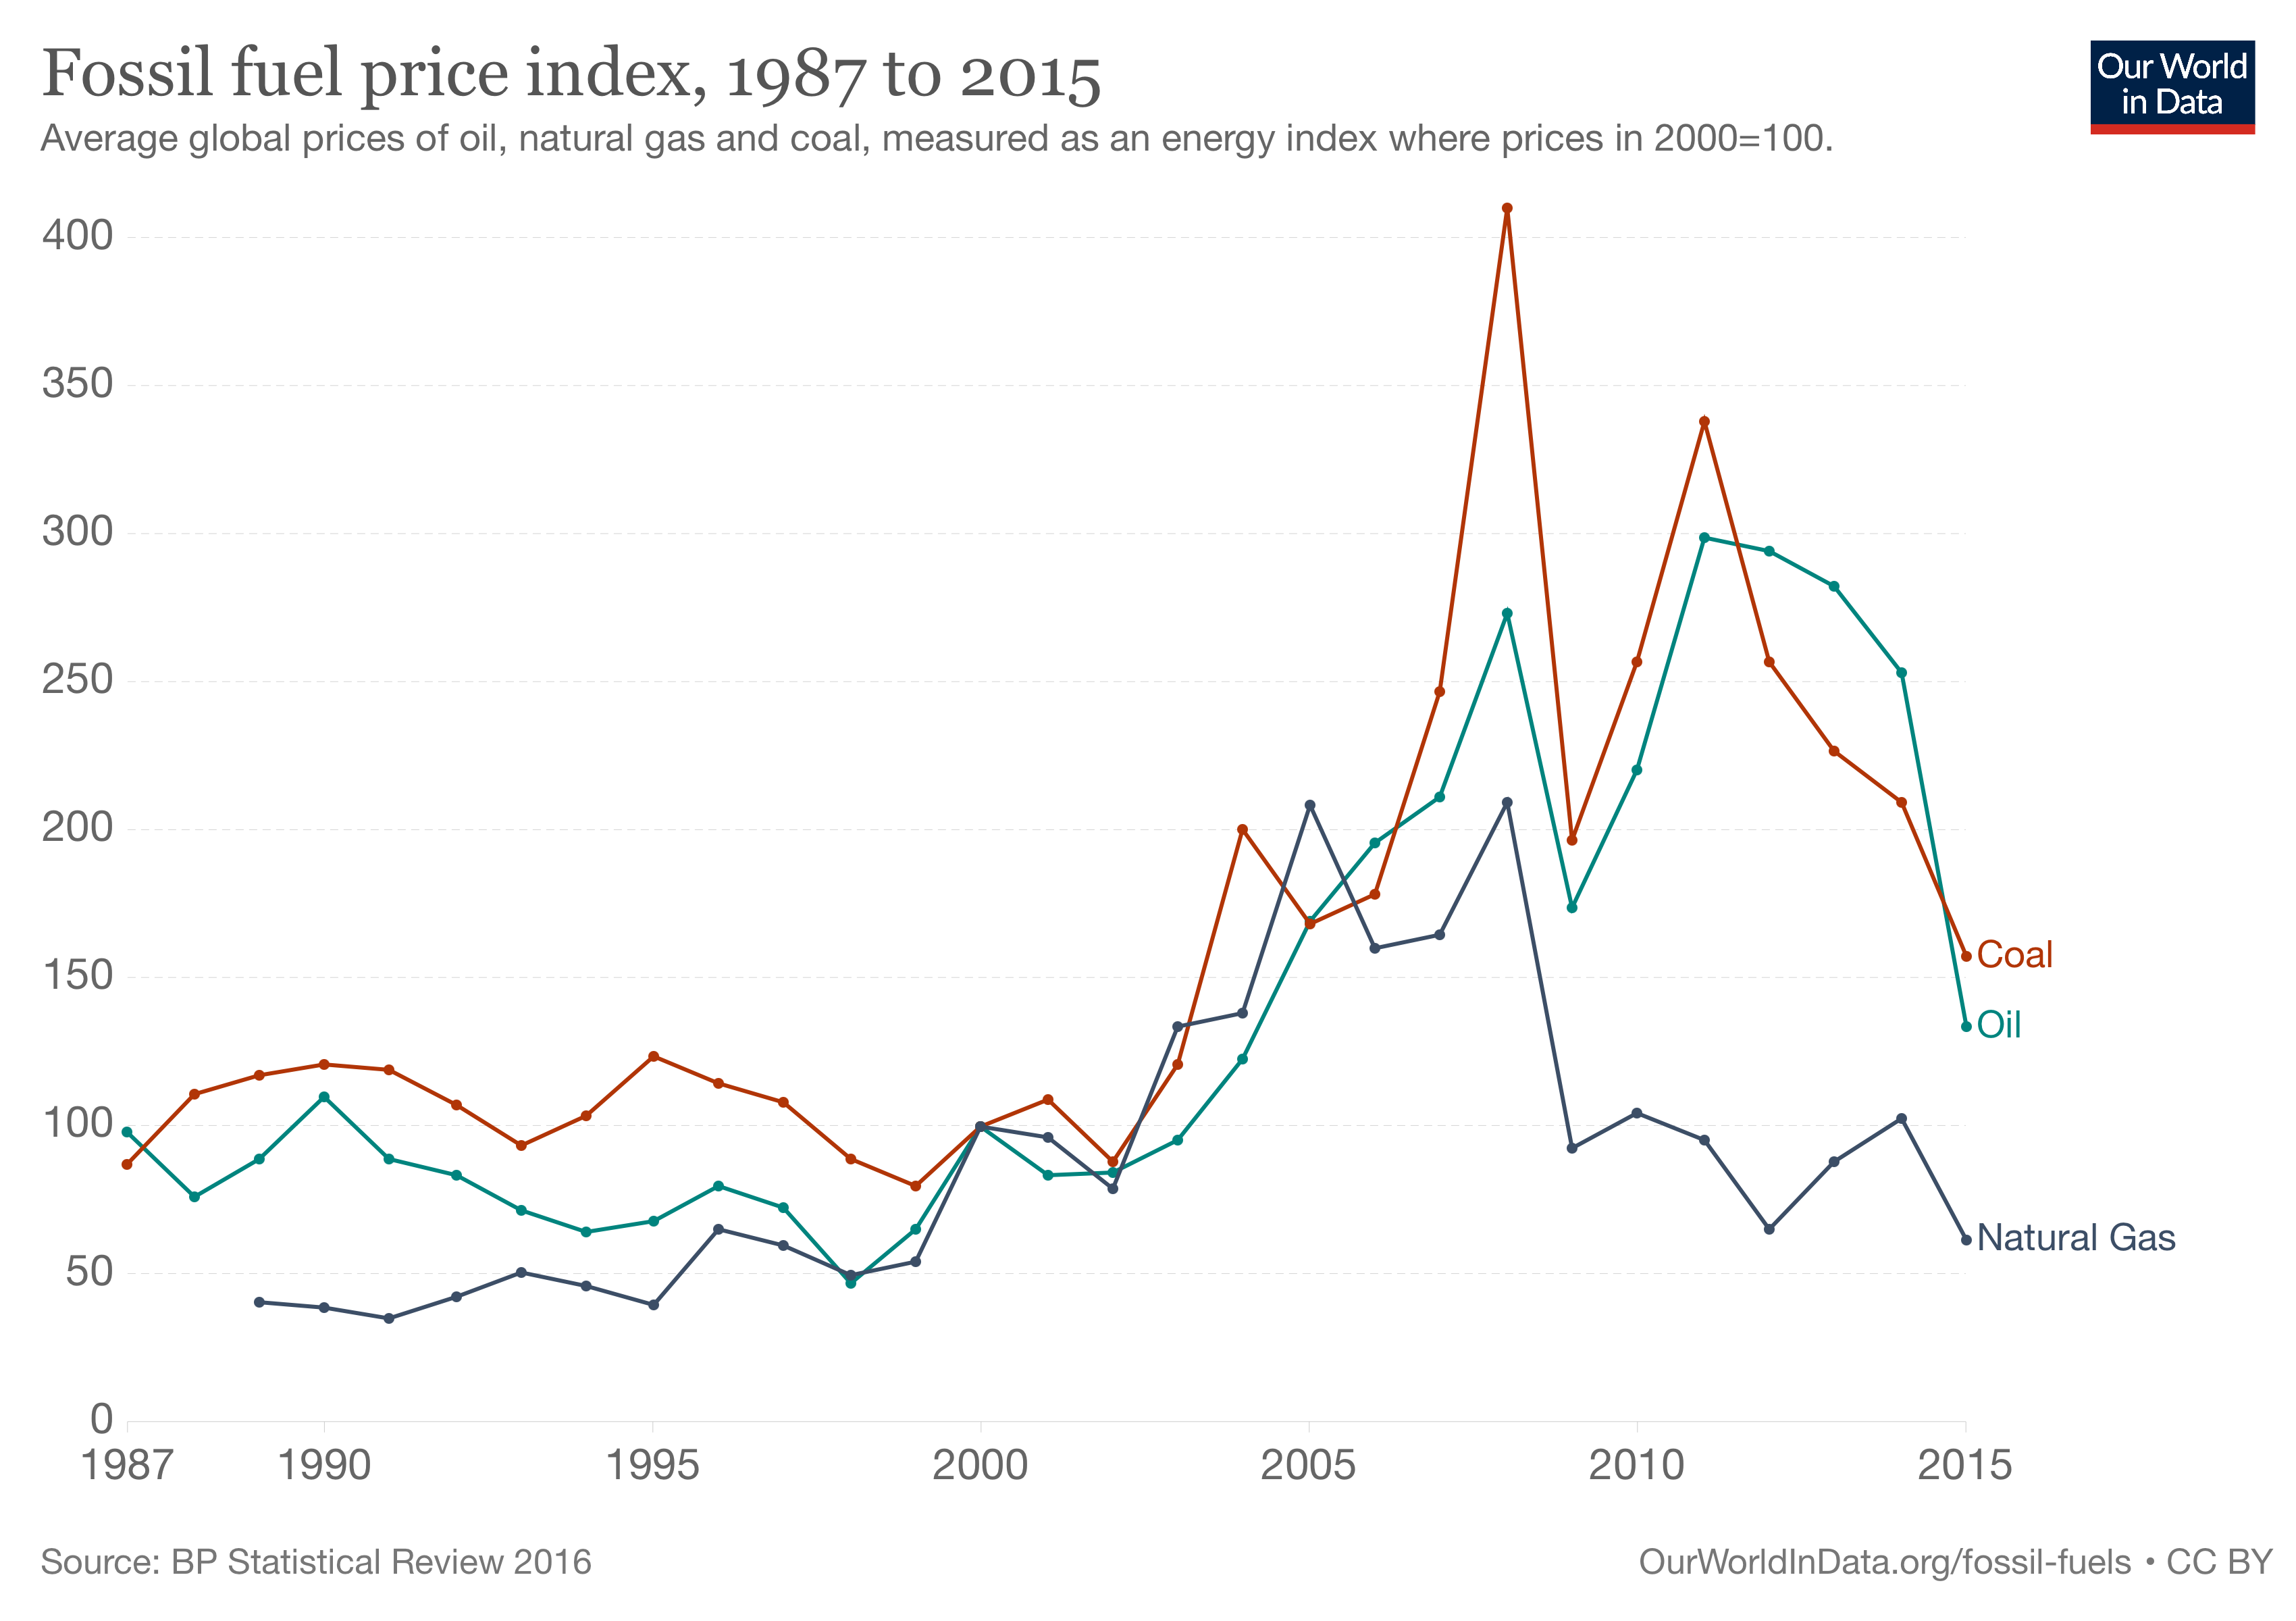
\includegraphics[scale=0.11]{img/intro_fossil-fuel-price-index.png}
\caption{Prices of different fossil fuels rose from 1987 to 2015 overall~\cite{BP2016bp}.}
\label{intro_fossil-fuel-price-index}
\end{figure} % Figure 1.2

Although we might not meet the complete depletion of non-renewable resources in the future 50 years, based on Hotelling’s "Economics of Exhaustible Resources", David Ricardo proposed that as the historical production stock accumulates, higher grade ores get depleted, and the producer resorts to lower grade ores, sustaining greater extraction costs~\cite{devarajan1981hotelling}. It means the extraction costs rise, and the price of the products based on ores will rise as well. Thus, we can assume that the price of most non-renewable resources, like oil, coal and gas, will rise since these have similar properties with ores. In fact, according to BP Statistical Review 2016, from 1987 to 2015 (from 1989 to 2015 for natural gas), the price of oil, coal and natural gas rose by approximately 36\%, 81\%, and 53\% overall (Figure~\ref{intro_fossil-fuel-price-index}). \\

The climate on the earth has changed throughout history. Just in the past 650,000 years, there were seven-cycle glaciers to advance and retreat. As shown in Figure~\ref{intro_co2-concentration-long-term}, however, atmospheric \ce{CO2} had never been above 300 parts per million until the year 1950. According to the paper from Nature, the climate has been changed differently from other periods that happened in the past 70 years~\cite{parmesan2003globally}. It has already had effects on the environment around us. Glaciers are shrinking, and ices are breaking up earlier on the lakes and rivers. Most climate scientists agree that it is human activities that cause global warming~\cite{epic337530}. The atmospheric concentration of \ce{CO2} has been risen for around 36\% since 1914 (see Figure~\ref{intro_co2-concentration-long-term}). As we know, \ce{CO2} is a significant component of the atmosphere. More than a third has increased atmospheric \ce{CO2} concentration since the Industrial Revolution began~\cite{epic337530}. More importantly, as shown in Figure \ref{intro_nasa_co2}, atmospheric \ce{CO2} has exceeded the highest level in the past 400,000 years, and it was 408.52 ppm in 2018. \\

\begin{figure}
\center
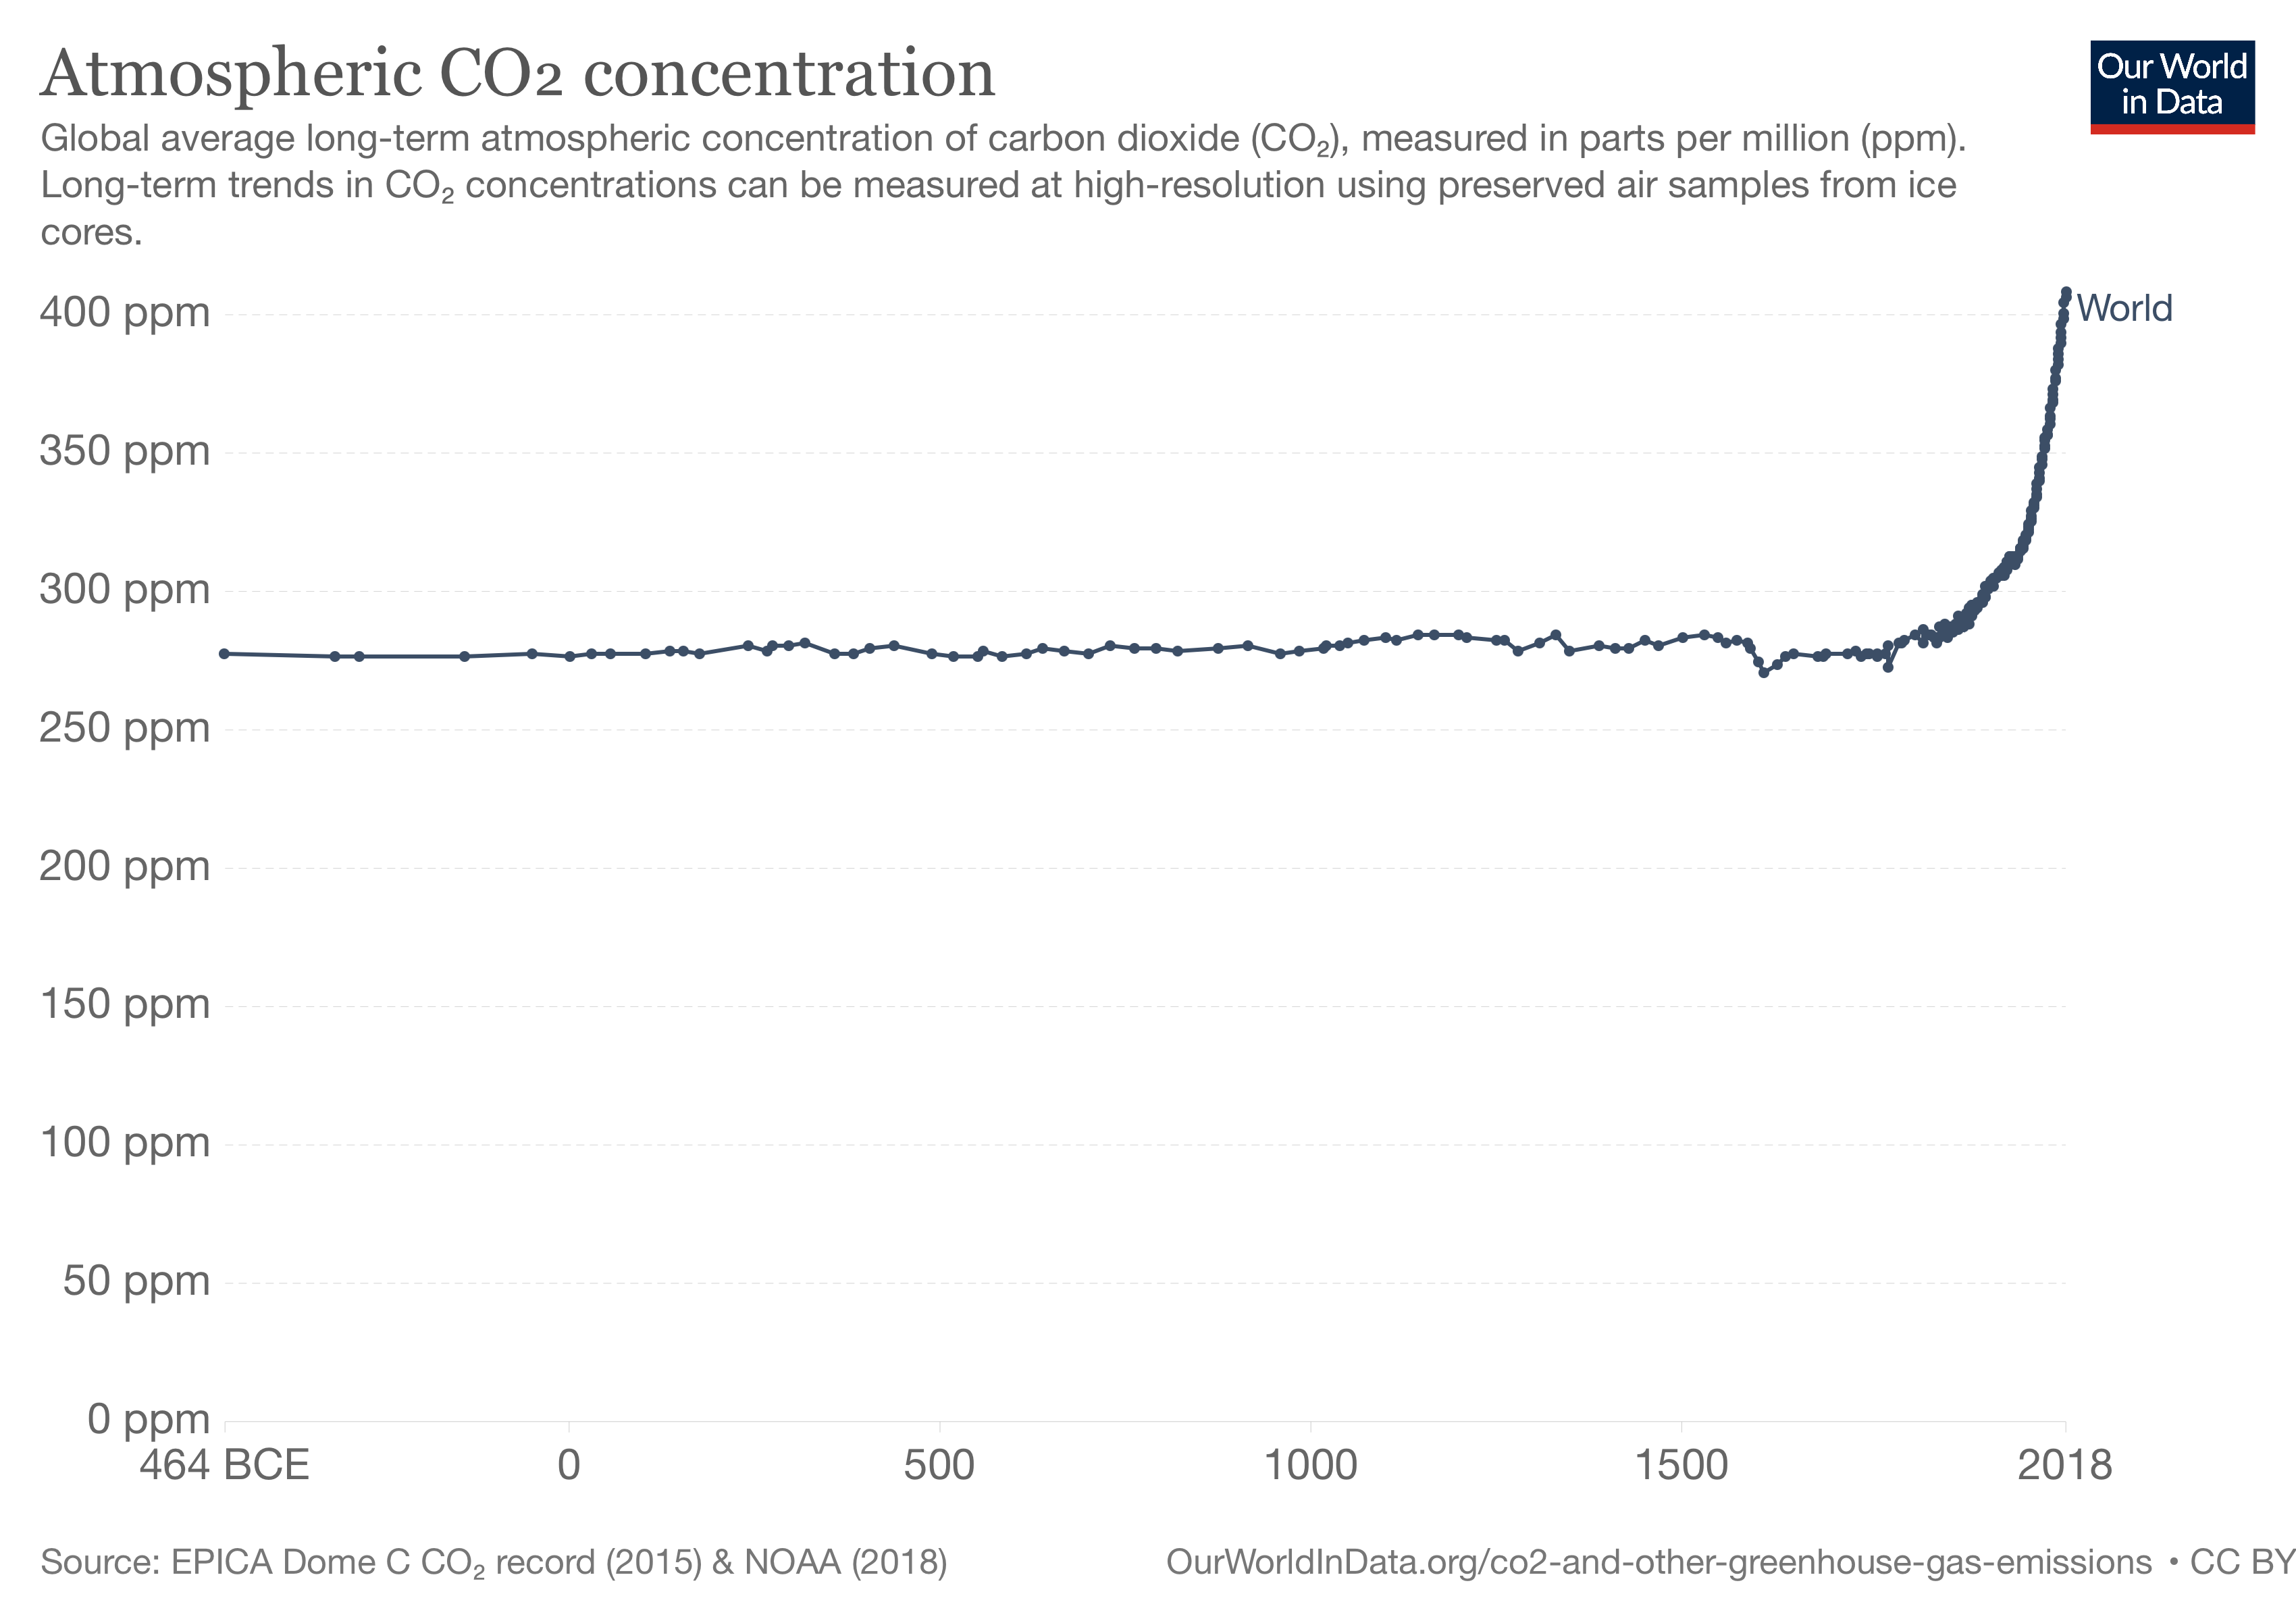
\includegraphics[scale=0.12]{img/intro_co2-concentration-long-term.png}
\caption{Atmospheric concentration of \ce{CO2} since 564 BCE~\cite{bereiter2015revision}. Atmospheric concentration of \ce{CO2} in 1914: 300.17ppm; Atmospheric concentration of \ce{CO2} in 2018: 408.52ppm.}
\label{intro_co2-concentration-long-term}

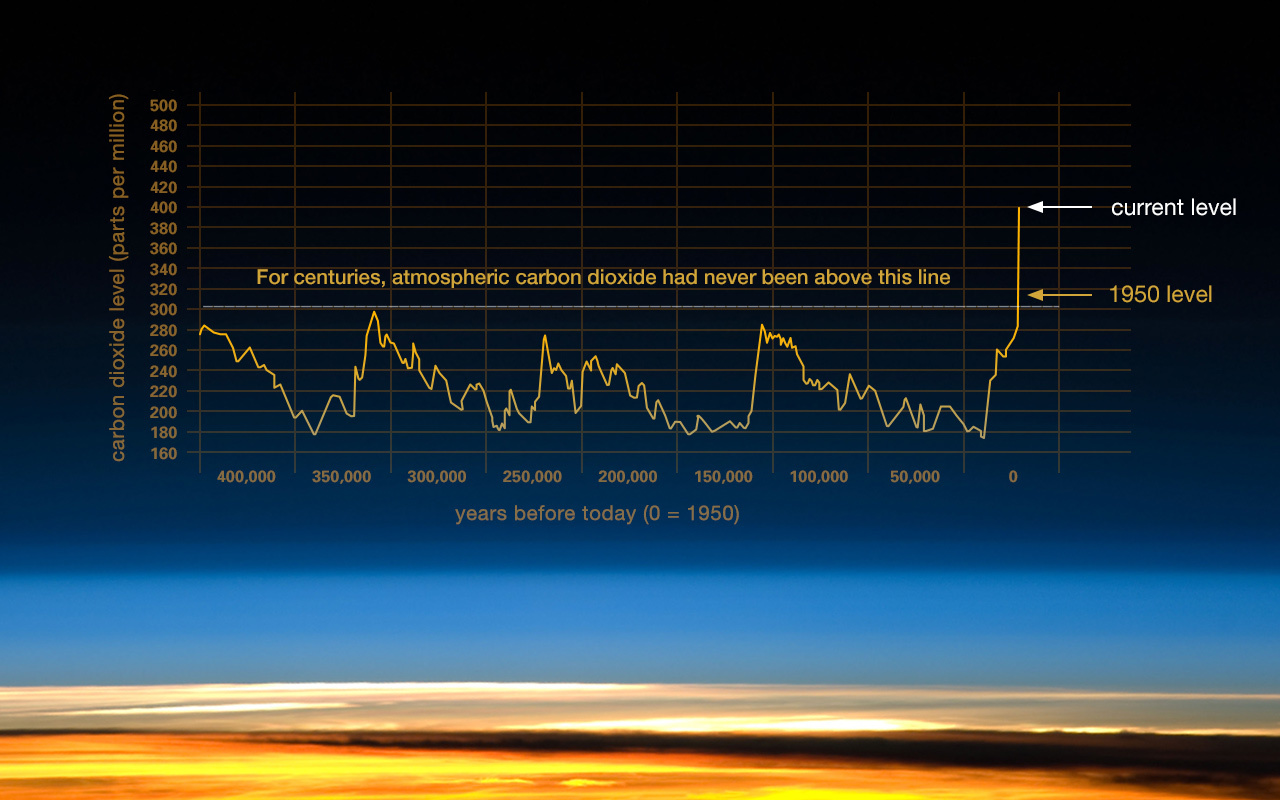
\includegraphics[scale=0.33]{img/intro_nasa_co2.jpeg}
\longcaption{The evidence that atmospheric \ce{CO2} has increased since the Industrial Revolution began}{\label{intro_nasa_co2} The evidence that atmospheric \ce{CO2} has increased since the Industrial Revolution began. Image courtesy: https://climate.nasa.gov/evidence}
\end{figure}


In summary, the rising energy demand and lack of energy supply may cause a short-term energy crisis. The finite resources of fossil energy will drive the price of electricity and consumer goods to rise. The burning of fossil energy will cause excessive emissions of greenhouse gases, leading to global warming. However, a door opens for cheaper but unpredictable renewable energy due to a more expensive fossil fuel. According to Paris Agreements~\cite{unies2015accord}, it is vital to reduce the emissions of fossil energy on a large scale in every sector of human activities. To respond to climate change, supporting the United Nations Sustainable Development Goals and taking urgent action to address climate change and its impact, the International Maritime Organization has formulated a timetable to reduce greenhouse gas emissions from international shipping.~\cite{joung2020imo} It pointed out that between 2030 and 2050, the carbon intensity of the fleet will be reduced by at least 70\%~\cite{joung2020imo}. Before 2050, the total annual greenhouse gas emissions will be reduced by at least 50\%, which requires a reduction of approximately 85\% of carbon dioxide per ship~\cite{joung2020imo}.\\ 

\subsection{Small-Boat Fleet and Emission Inventory}
In 2018, total shipping \ce{CO2} emissions increased to 1056 million tonnes compared to 962 million tonnes in 2012~\cite{IMO2021Fourth}.
In 2016, total \ce{CO2} emissions of the industrial fishing sector were 159 million tonnes, and the small-scale fishing sector emitted 48 million tonnes~\cite{GREER2019103382}. Suppose the increase rate of \ce{CO2} in 2018 was the same as the rate in 2016, and the ratio of the number of small boats and the number of boats can be approximate as the ratio of the number of small fishing boats and the number of fishing boats. Then in 2018, the total \ce{CO2} emissions for the small boat fleet can be calculated as 318.8 million tonnes.\\

Small vessels are classified as those smaller than 24 meters~\cite{uk2021Operational}. Knowing the emissions inventory of the shipping sector can help to understand what measures need to be taken to enable the industry to start the road to full decarbonization. Although it is possible to calculate large vessels from the international registry system and use the satellite data sent from the ship's transponder to account for the numbers of the large vessels~\cite{IMO2021Fourth}, the small vessels depend on the national registration system, and their operation is assumed. In addition, there are many types of small vessels fleets such as machinery (e.g. fishery, people carrier, etc.), hull shape and structure, and the activities of owners and operators. The diverse small boat fleet operational profile is increasing the challenge of accurately accounting for their emission inventories.\\

Emissions from the global fishing industry grew by 28\% between 1990 and 2011, with a minor coinciding increase in production; however, marine fisheries are typically excluded from international assessments of \ce{CO2} or are generalized based on a limited number of case studies~\cite{parker2018fuel}. Developed economies such as the UK have a national registry~\cite{uk2021registration} that allows to have a sense of the level of small boat activity and hence infer the \ce{CO2} emissions.\\

However, in developing countries, it tends to be a mixed bag on the level of precision and availability. For instance, in Mexico, only fishing vessels are counted into registry~\cite{Mexico2021RegisteredVessels}. Still, it is difficult to know where they are located. Besides, the rest of the small-boat fleets are not considered. In all, Mexico does not have a regional \ce{CO2} inventory considering the small-boat fleet. Therefore, quantifying the number of small-boat fleets will allow a better precision of where the emissions are being emitted and will be the focus of understanding the emission inventory of the shipping sector.\\


Observing the shipping activity in the Gulf of California is essential due to its unique geographical location, conformation, and biophysical environment ~\cite{LLUCHCOTA20071, munguia2018ecological, MARINONE2012133}. In the Gulf of California, there is the largest fish producing state (Sonora) in Mexico~\cite{MELTZER2006222} and the most prominent sports fishing destination (Los Cabos, Baja) in Mexico~\cite{hernandez2012economic}. Besides, the Gulf of California has a faster shipping route to mainland Mexico than from Yucatán Peninsula.\\

\subsection{Bringing Image Recognition in Satellite Images Detection}

\section{Research Questions}


\section{Thesis Outline}


\section{Contributions}